%% -*- TeX-engine: luatex; ispell-dictionary: "english" -*-

\documentclass[unicode,11pt]{beamer}

\usepackage{algpseudocode}
\usepackage{tikz}
\usetikzlibrary{bayesnet}
\usetikzlibrary{arrows}

\usepackage{mathtools}  %% for \underbrace

\usepackage{subcaption}
\captionsetup{compatibility=false}

\PassOptionsToPackage{obeyspaces}{url}

\usetheme{Pittsburgh}
\usecolortheme{beaver}

\newenvironment{stopperenv}{\only{\setbeamercolor{local structure}{fg=darkred}}}{}

\setbeamercolor{frametitle}{fg=black,bg=white}
\setbeamerfont{frametitle}{size=\Large}
\setbeamertemplate{footline}[frame number]
\setbeamertemplate{frametitle continuation}{(\insertcontinuationcount)}
\setbeamertemplate{caption}{\insertcaption}
\setbeamertemplate{enumerate items}[default]
\setbeamertemplate{frametitle}{\hfill\insertframetitle\vskip-6pt\hrulefill}

\setbeamercovered{dynamic} % overlays not yet revealed will faintly appear
\beamertemplatenavigationsymbolsempty

\usepackage{fontspec}
\setmainfont{PT Serif}
\setsansfont{PT Sans}
\setmonofont[Ligatures=NoCommon]{PT Mono}
\defaultfontfeatures{Ligatures=TeX}

% sans serif for headings
\setbeamerfont*{block title}{family=\sffamily,series=\bfseries}

%\usepackage{microtype}


\newcommand{\theme}[1]{%
  \centering\fontsize{36pt}{1em}\color{darkred}{\selectfont{#1}}
}

\usepackage{polyglossia}
\setdefaultlanguage{english}
\usepackage{csquotes}

\usepackage[normalem]{ulem}

\usepackage{hyperref}
\hypersetup{
	colorlinks=true,
    linkcolor=darkred,
    urlcolor=darkred,
    citecolor=darkred
}

\makeatletter
\let\@mycite\@cite
\def\@cite#1#2{{\hypersetup{linkcolor=darkred}[{#1\if@tempswa , #2\fi}]}}
\makeatother

\usepackage{caption}
\captionsetup[figure]{labelformat=empty}

\usepackage{amsmath}
\usepackage{amssymb}
\DeclareMathOperator*{\argmin}{arg\,min}
\DeclareMathOperator*{\argmax}{arg\,max}

\newcommand{\op}[1]{\operatorname{#1}}


\title{Variational Auto-Encoder \\
  \& \\
  Normalizing Flows}
\author{S. Lebedev, E. Tuzova}
%\institute{JetBrains}
\date{\today}

\begin{document}

% 1
\begin{frame}[plain,noframenumbering]
  \maketitle
\end{frame}


\begin{frame}{Motivation\footnote{Slide credit: G. Hinton, CSC2515, <<Continuous
      Latent Variable Models>>.}}
  \begin{center}
    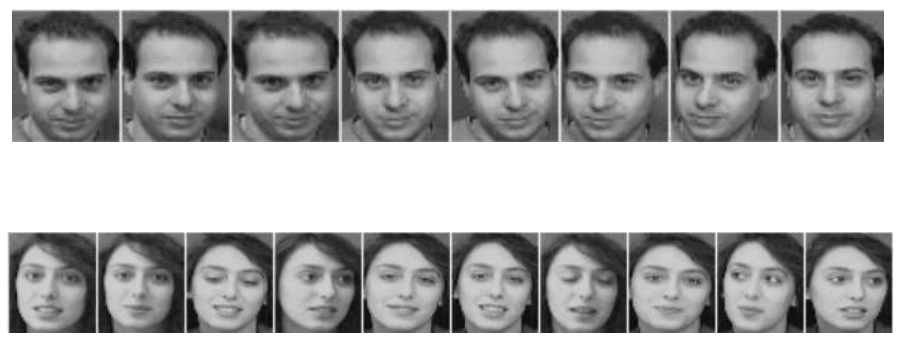
\includegraphics[width=.8\textwidth]{images/motivation}
  \end{center}

  What are the underlying \hl{hidden} factors in these two datasets?
\end{frame}

% 2
\begin{frame}[fragile]{Problem scenario}
  \begin{center}
    \begin{minipage}[t]{.3\linewidth}
      \begin{tikzpicture}[baseline=0]
        \node[latent]            (z) {$\mathbf{z}$};
        \node[obs, below=of z]   (x) {$\mathbf{x}$};
        \node[const, right=of z] (t) {$\theta$};
        \node[const, left=of x, xshift=2em]   (lfantom) {};
        \node[const, right=of x, xshift=-2em] (rfantom) {};

        \edge {z} {x};
        %\draw (x) edge [->,dashed,bend left=45] (z);
        \edge {t} {x,z};

        \plate {xz} {(x)(z)(lfantom)(rfantom)} {$~N$};
      \end{tikzpicture}
    \end{minipage}
    \begin{minipage}[t]{.55\linewidth}
      % $X = \left\{ x^{(i)}\right\}_{i=1}^N~-$ dataset\\
      $x$ --- observed variables\\
      $z$ --- \hl{continuous} latent variables\\
      $\theta$ --- model parameters\\
      % $\phi~-$ variational parameters\\
      $p(x, z|\theta) = p(x|z, \theta) p(z|\theta)$ %--- joint p.d.f.\\
    \end{minipage}
  \end{center}

  \begin{itemize}
  \item Goal: fast approximate posterior inference for the latent variables
    in the ``real-world'' scenario.
  \item Specifically when
    \begin{itemize}
    \item non-conjugate distributions are involved,
    \item so the evidence and posterior for latent variables are both
      \hl{intractable}.
    \item Mean-field VB is \hl{not applicable} because the integrals
      required are intractable as well.
    \end{itemize}
  \end{itemize}

  %% TODO: scalable as well? or expand on fast.
\end{frame}


\begin{frame}{What are the options?}
  \begin{itemize}
  \item MCMC
    \begin{itemize}
    \item slow for large-scale problems,
    \item diagnosing convergence is an issue.
    \end{itemize}
  \item MAP
    \begin{itemize}
    \item easy to overfit the data,
    \item especially in the case of high-dimensional $z$.
    \end{itemize}
  \item VB
    \begin{itemize}
    \item mean-field cannot be applied directly,
    \item but still a good idea,
    \item maybe.
    \end{itemize}
  \end{itemize}
\end{frame}


\begin{frame}{The plan}
  \begin{enumerate}
  \item[] \hl{tl;dr} reduce inference problem to stochastic optimization.
    \vspace{1em}
  \item Approximate the posterior with a neural net
    $q(z|x, \phi)$, where $\phi$ --- variational parameters.
  \item Lower bound the evidence using $q(z|x, \phi)$.
  \item Construct an estimator of the ELBO which can be
    optimized jointly w.r.t. $\phi$ and $\theta$.
  \item Use stochastic gradient ascent to optimize the estimator.
  \item Profit.
  \end{enumerate}
\end{frame}


\begin{frame}{ELBO}
  Having $q(z|x, \phi)$ we can deconstruct the evidence into
  \begin{align*}
    \log p(x|\theta)
    &= \log \int p(x, z|\theta) dz
     = \log \int q(z|x, \phi) \frac{p(x, z|\theta)}{q(z|x, \phi)} dz \\
    &= \KL{q(z|x, \phi)}{p(z|x, \theta)} + \mathcal{L}(\theta, \phi; x) \\
    &\ge \mathcal{L}(\theta, \phi; x)
  \end{align*}
  where the lower bound is given by
  \begin{align*}
    \mathcal{L}(\theta, \phi; x)
    &= \E{q(z|x, \phi)}{\log p(x, z|\theta) - \log q(z|x, \phi)} \\
    &= \E{q(z|x, \phi)}{\log p(x|z, \theta)}
     - \KL{q(z|x, \phi)}{p(z|\theta)}
  \end{align*}

  % \begin{itemize}
  %   \item $q(z|x)$ is not necessarily factorial
  %   \item Parameters $\phi$ are not computed from some closed-form expectation
  % \end{itemize}
\end{frame}


\begin{frame}{Optimizing the ELBO}
  \begin{itemize}
  \item Want to optimize the lower bound w.r.t \hl{both} $\theta$ and $\phi$.
  \item Just-do-it approach:
    \begin{align*}
      \grad_\theta \mathcal{L}(\theta, \phi; x)
      &= \grad_\theta \E{q(z|x, \phi)}{\log p(x, z|\theta) - \log q(z|x, \phi)} \\
      &= \E{q(z|x, \phi)}{\grad_\theta \log p(x, z|\theta)} \\
      &\approx \frac{1}{S} \sum\limits_{s = 1}^S
           \grad_\theta \log p(x, z^{(s)}|\theta) \\
      \grad_\phi \mathcal{L}(\theta, \phi; x)
      &= \grad_\phi \E{q(z|x, \phi)}{\log p(x, z|\theta) - \log q(z|x, \phi)}
    \end{align*}
  \item How to deal with gradients of the form $\grad_\phi \E{q(z|\phi)}{f(z)}$?
  \end{itemize}
\end{frame}


\begin{frame}{Na\"ive MCMC estimator of $\grad_\phi \E{q(z|\phi)}{f(z)}$}
  \begin{align*}
    \grad_\phi \E{q(z|\phi)}{f(z)}
    &= \grad_\phi \int q(z|\phi) f(z) dz
     = \int f(z) \grad_\phi q(z|\phi) dz \\
    &= \int f(z) q(z|\phi) \grad_\phi \log q(z|\phi) dz
  \end{align*}
  where the last line is due to the \hl{log derivative trick}
  \footnote{%
    \url{http://blog.shakirm.com/2015/11/machine-learning-trick-of-the-day-5-log-derivative-trick}}
  $$
  \grad_\phi \log q(z|x, \phi) = \frac{\grad_\phi q(z|x, \phi)}{q(z|x, \phi)}
  $$
  Proceeding further we obtain
  \begin{align*}
    \grad_\phi \E{q(z|\phi)}{f(z)}
    &= \E{q(z|x, \phi)}{f(z) \grad_\phi \log q(z|\phi)} \\
    &\approx \frac{1}{S} \sum\limits_{s = 1}^S f(z^{(s)}) \grad_\phi \log q(z^{(s)}|\phi)
    \to \op{:(}
  \end{align*}

  %% TODO: covariance of sample mean is Cov(mean(X)) = Cov(X) / S,
  %% thus if the diagonal entries in Cov(X) are large, S must be
  %% large as well.
\end{frame}


\begin{frame}{Reparametrization trick%
  \footnote{\url{http://blog.shakirm.com/2015/10/machine-learning-trick-of-the-day-4-reparameterisation-tricks}}}
  \begin{itemize}
  \item Introduce an auxilary noise variable $\epsilon$ \hl{independent} of
    $\phi$.
  \item Express $z$ as a \hl{determinisitic} transformation of $\epsilon$
    \hl{differentiable} w.r.t. $\phi$
    $$
    z = g(\epsilon, x; \phi)
    \qquad
    \epsilon \sim p(\epsilon)
    $$
  % \item Plug the transformed variable into the expectation
  %   $$
  %   \E{q(z|x, \phi)}{f(z)}
  %   = \E{p(\epsilon)}{f(g(\epsilon, x; \phi)}
  %   \approx \frac{1}{S} \sum\limits_{s = 1}^S f(g(\epsilon^{(l)}, x; \phi))
  %   $$
  \item  Example: let $q(z|\phi) = \mathcal{N}(z|\mu, \sigma^2)$ and
    $\phi = (\mu, \sigma^2)$ then
    \begin{align*}
      \grad_\phi \E{q(z|\phi)}{f(z)}
      &= \E{\mathcal{N}(\epsilon|0, 1)}{\grad_\phi f(\mu + \sigma \epsilon)} \\
      &\approx \frac{1}{S} \sum\limits_{s = 1}^S \grad_\phi f(\mu + \sigma \epsilon^{(s)})
    \end{align*}
    where $z = \mu + \sigma\epsilon$ and $\epsilon \sim \mathcal{N}(0, 1)$.
  \end{itemize}
\end{frame}


\begin{frame}{SGVB estimator}
  \begin{itemize}
  \item In general
    \begin{align*}
      \mathcal{L}(\theta, \phi; x)
      &= \E{q(z|x, \phi)}{\log p(x, z|\theta) - \log q(z|x, \phi)} \\
      &\approx \frac{1}{S} \sum\limits_{s = 1}^S
            \log p(x, z^{(s)}|\theta) - \log q(z^{(s)}|x, \phi) \\
      &\triangleq \widetilde{\mathcal{L}}(\theta, \phi; x, z)
    \end{align*}
    where $z^{(s)} = g(\epsilon^{(s)}, x; \phi)$ and $\epsilon^{(s)} \sim p(\epsilon)$.
  \item If $\KL{q(z|x, \phi)}{p(z|\theta)}$ is tractable
    \begin{align*}
      \mathcal{L}(\theta, \phi; x)
      &= \E{q(z|x, \phi)}{\log p(x|z, \theta)} - \KL{q(z|x, \phi)}{p(z|\theta)} \\
      &\approx \frac{1}{S} \sum\limits_{s = 1}^S \log p(x|z^{(s)}, \theta)
       - \KL{q(z|x, \phi)}{p(z|\theta)} \\
      &\triangleq \widetilde{\mathcal{L}}(\theta, \phi; x, z)
    \end{align*}
  \end{itemize}
\end{frame}


\begin{frame}{AEVB algorithm \cite{kingma2013auto}}
  \centering
  \begin{algorithmic}
    \State $\alpha \gets$ set learning rate
    \State $\theta, \phi \gets$ initialize parameters
    \Repeat
       \State $x \gets$ random datapoint or minibatch
       \hl{\State $\epsilon \gets$ random samples from $p(\epsilon)$}
       \hl{\State $z \gets g(\epsilon, x; \phi)$}
       \State $g_\theta, g_\phi \gets \grad_{\phi, \theta} %
           \mathcal{\widetilde{L}}(\theta, \phi; x, z)$
       \State $\theta \gets \theta + \alpha g_\theta$
       \State $\phi \gets \phi + \alpha g_\phi$
    \Until convergence \\
    \Return $\theta$, $\phi$
  \end{algorithmic}
\end{frame}


\begin{frame}{Variational auto-encoder}
  \begin{center}
    \begin{minipage}[t]{.3\linewidth}
      \begin{tikzpicture}[baseline=1em]
        \node[latent]            (z) {$z$};
        \node[obs, below=of z]   (x) {$x$};
        \node[const, right=of z] (t) {$\theta$};
        \node[const, left=of z]  (p) {$\phi$};
        \node[const, left=of x, xshift=2em]   (lfantom) {};
        \node[const, right=of x, xshift=-2em] (rfantom) {};

        \edge {z} {x};
        \draw (x) edge [->,dashed,bend left=45] (z);
        \draw (p) edge [->,dashed] (z);
        \edge {t} {x,z};

        \plate {xz} {(x)(z)(lfantom)(rfantom)} {$~N$};
      \end{tikzpicture}
    \end{minipage}
    \begin{minipage}[t]{.55\linewidth}
      \begin{align*}
        p(z|\theta) &= \mathcal{N}(z|0, \mathbf{I}) \\
        p(x|z, \theta) &= \mathcal{N}(x| \mu(z), \sigma^2(z) \mathbf{I}) \\
        q(z|x, \phi) &= \mathcal{N}(z| M(x), S^2(x) \mathbf{I}) \\
      \end{align*}
    \end{minipage}
  \end{center}

  \begin{itemize}
  \item The parameters $M(x)$ and $S^2(x)$ are computed by a neural net,
    which assigns each value of $x$ a \hl{distribution} over $z$.
  \item The parameters $\mu(z)$ and $\sigma^2(z)$ are computed by a
    \hl{different} neural net, mapping $z$ to a distribution over $x$.
  \end{itemize}
\end{frame}


\begin{frame}{VAE illustrated}
  \centering
  \begin{tikzpicture}
    \node[obs]                 (x1) {$x$};
    \node[latent, below=of x1] (z) {$z$};
    \node[latent, left=of z]   (e) {$\epsilon$};
    \node[obs, below=of z]     (x2) {$x$};

    \node[below=of e, yshift=2em, align=center] {injected\\noise};
    \path (z) edge [->] node [midway, right, xshift=2em]
        {$p(x|z, \theta)$ \hl{aka} decoder} (x1);
    \path (x2) edge [->, dashed] node [midway, right, xshift=2em]
        {$q(z|x, \phi)$ \hl{aka} encoder} (z);
    \edge {e} {z};
  \end{tikzpicture}

  $$
  \mathcal{L}(\theta, \phi; x)
  = \underbrace{\E{q(z|x, \phi)}{\log p(x|z, \theta)}}_{\text{negative reconstruction error}}
  - \underbrace{\KL{q(z|x, \phi)}{p(z|\theta)}}_{\text{regularizer}}
  $$
\end{frame}


\begin{frame}{Experiments: Frey faces}
  \begin{figure}
    \centering
    \begin{subfigure}[b]{.4\linewidth}
      \centering
      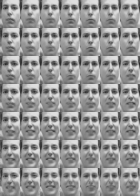
\includegraphics[width=.8\linewidth]{images/vae_frey_B100_E4000_N560_L2_H200_C_manifold_8}
      \caption{Learned data manifold}
    \end{subfigure}
    \hspace{1em}
    \begin{subfigure}[b]{.4\linewidth}
      \centering
      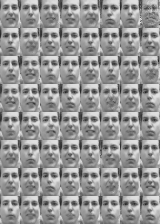
\includegraphics[width=.8\linewidth]{images/vae_frey_B100_E4000_N560_L2_H200_C_sample_64}
      \caption{Random samples}
    \end{subfigure}
  \end{figure}
\end{frame}


\begin{frame}{Experiments: MNIST}
  \begin{figure}
    \centering
    \begin{subfigure}[b]{.4\linewidth}
      \centering
      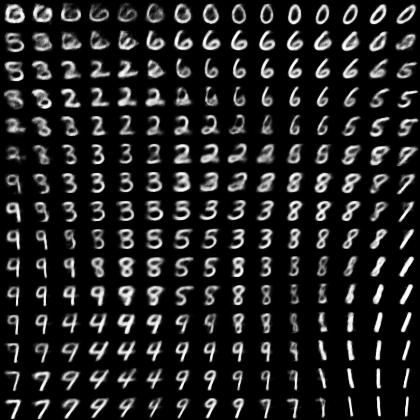
\includegraphics[width=\linewidth]{images/vae_mnist_B200_E1000_N784_L2_H400_D_manifold_16}
      \caption{Learned data manifold}
    \end{subfigure}
    \hspace{1em}
    \begin{subfigure}[b]{.4\linewidth}
      \centering
      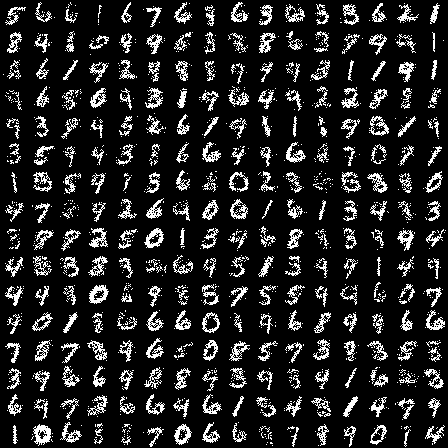
\includegraphics[width=\linewidth]{images/vae_mnist_B200_E1000_N784_L2_H400_D_sample_256}
      \caption{Random samples}
    \end{subfigure}
  \end{figure}
\end{frame}


\begin{frame}[c,noframenumbering,plain]
  \centering\fontsize{24pt}{1em}\color{darkred}{\selectfont{What is wrong with VAE?}}
  %% Answer: q(z|x) is diag. gaussian.
\end{frame}


\begin{frame}[fragile]{Normalizing flows}
  We want to specify a \hl{complex} joint distribution over z.\\
  ~\\
  $z$ --- random variable with distribution $q(z)$\\
  $f$ --- invertible parametric function\\
  ~\\
  Transformation of random variables: $\tilde{z} = f(z)$, ~$f^{-1}(\tilde{z}) = z$\\
  $$
  q(\tilde{z})
  = q(f^{-1}(\tilde{z})) \left\vert \det \frac{\partial f^{-1}(\tilde{z})}{\partial \tilde{z}} \right\vert
  = q(z) \left\vert \det \frac{\partial f(z)}{\partial z} \right\vert^{-1}
  $$ \\

\end{frame}


\begin{frame}[fragile]{Normalizing flows}

  Chaining together a sequence: $z_K = f_K ( f_{K−1} ( \cdots f_2 ( f_1(z_0)))$\\
  $$\log q_K(z_K) = \log q_0(z_0) − \sum_{k=1}^K \log \left\vert \det \frac{\partial f_k}{\partial z_k} \right\vert $$

  Law of the unconscious statistician:\\
  $$\mathbb{E}_{q_K} \left[g(z_K)\right] = \mathbb{E}_{q_0} \left[ g(f_K ( f_{K−1} ( \cdots f_2 ( f_1(z_0))) \right] $$
\end{frame}


\begin{frame}[fragile]{Planar flow}
  \textcolor{darkred}{Family of transformations:} ~$f(z) = z + uh\left( w^T z + b \right)$\\
  $$ \left\vert \det \frac{\partial f(z)}{\partial z} \right\vert = \left\vert 1 + u^T \psi(z)
  \right\vert ~~~\text{where}~~~ \psi(z) = h'(w^Tz + b)w$$ \\
  $$\log q_K(z_K) = \log q_0(z_0) − \sum_{k=1}^K \log \left\vert 1 + u^T \psi(z) \right\vert $$\\
  ~\\
  Chaining transformations gives us a rich family of posteriors.
  \begin{center}
    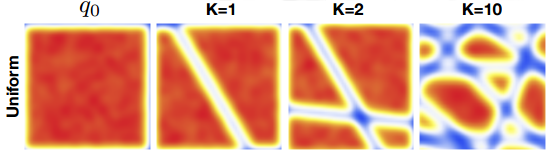
\includegraphics[width=.8\textwidth]{images/planar_flow}
  \end{center}
\end{frame}


\begin{frame}[fragile]{Radial flow}
  \textcolor{darkred}{Family of transformations:} ~$f(z) = z + \beta h(\alpha, r)(z-z_0)$\\
  \hspace{12em}$r = \vert z-z_0 \vert$,~~~ $h(\alpha, r) = \frac{1}{\alpha + r}$\\
  ~\\
  $\left\vert \det \frac{\partial f}{\partial z} \right\vert = [1 + \beta h(\alpha, r)]^{(d-1)}
  [1 + \beta h(\alpha, r) + h'(\alpha, r) r]$\\
  ~\\
  Chaining transformations gives us a rich family of posteriors.
  \begin{center}
    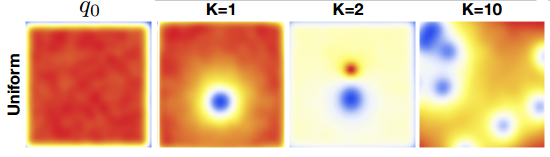
\includegraphics[width=.8\textwidth]{images/radial_flow}
  \end{center}
\end{frame}


\begin{frame}{Representative power of normalizing flows}
  \begin{itemize}
  \item Choose a non-trivial density $p(z) \propto \exp[-U(z)]$.
  \item Example:
    $$
    U(z) = \frac{1}{2} \left( \frac{z_2 - w_1(z)}{0.4} \right)
    \qquad
    w_1(z) = \sin \frac{2 \pi z_1}{4}
    $$
  \item Approximate the density with a flow by optimizing
    \begin{align*}
      \KL{q(z_K)}{p(z)}
      &= \int q(z_K) \log \frac{q(z_K)}{p(z)} dz_K \\
      &= \E{q(z_K)}{\log q(z_K) - (-U(z) + \op{const}(z_K))} \\
      &\approx \frac{1}{S} \sum\limits_{s = 1}^S \left( \log q(z_K) + U(z) \right) + \op{const}(z_K)
    \end{align*}
  \end{itemize}
\end{frame}


\begin{frame}[fragile]{Representative power of \hl{planar} flows}
  \begin{center}
    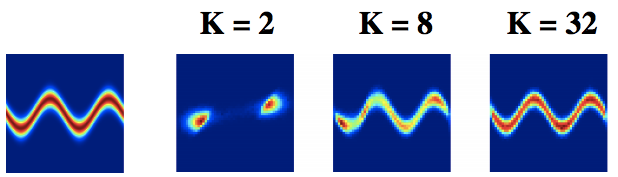
\includegraphics[width=.8\textwidth]{images/normalizing_flow}
  \end{center}

  \begin{center}
    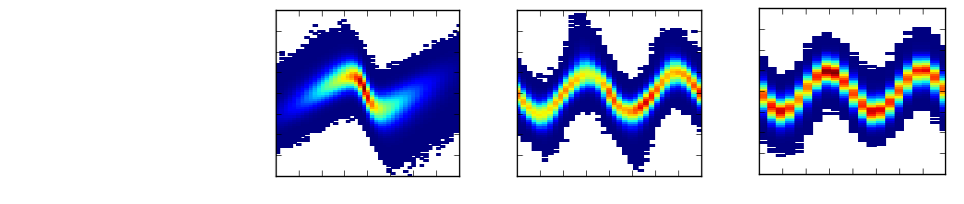
\includegraphics[width=.8\textwidth]{images/normalizing_flow1}
  \end{center}
\end{frame}


\begin{frame}{VAE and normalizing flows}
  \centering
  \begin{tikzpicture}
    \node[obs]                 (x1) {$x$};
    \node[latent, below=of x1] (zK) {$z_K$};
    \node[latent, below=of zK] (z0) {$z_0$};
    \node[latent, left=of z0]  (e) {$\epsilon$};
    \node[obs, below=of z0]    (x2) {$x$};

    \node[below=of e, yshift=2em, align=center] {injected\\noise};
    \path (zK) edge [->] node [midway, right, xshift=2em]
        {$p(x|z_K, \theta)$ \hl{aka} decoder} (x1);
    \path (x2) edge [->, dashed] node [midway, right, xshift=2em]
        {$q(z_0|x, \phi)$ \hl{aka} encoder} (z0);
    \path (z0) edge [->] node [midway, right, xshift=2em]
        {normalizing flow} (zK);
    \edge {e} {z0};
  \end{tikzpicture}
\end{frame}


% 21
\begin{frame}[fragile]{ELBO with planar normalizing flow}
  \begin{align*}
  \mathcal{L}(\theta, \phi, x) &= \mathbb{E}_{q(z|x, \phi)} \left[ \log p(x, z | \theta) - \log q(z | x, \phi) \right] \\
  &= \mathbb{E}_{q_K(z_K| \theta)} \left[ \log p(x, z_K | \theta) - \log q(z_K | \hl{\phi}) \right] \\
  &= \mathbb{E}_{q_0(z_0|x, \hl{\phi})} \bigg[ \log p(x, z_K| \theta) - \log q_0(z_0| x, \hl{\phi})  \\
  &\hspace{6em} + \sum_{k=1}^K \log \left\vert \det
  \frac{\partial f_k}  {\partial z_k} \right\vert \bigg]
  \end{align*}
\end{frame}


% 22
\begin{frame}[fragile]{NFVB algorithm \cite{rezende2015variational}}
  \begin{algorithmic}
    \State $\alpha \gets$ set learning rate
    \State $\theta, \phi \gets$ initialize parameters
    \Repeat
       \State $x \gets$ random datapoint or minibatch
       \State $\epsilon \gets$ random samples from $p(\epsilon)$
       \hl{\State $z_0 \gets g(\epsilon, x; \phi)$}
       \hl{\State $z_K \gets f_K(f_{K-1}(\cdots f_1(z_0)))$}
       \State $g_\theta, g_\phi \gets \grad_{\phi, \theta} %
           \mathcal{\widetilde{L}}(\theta, \phi; x, z_K)$
       \State $\theta \gets \theta + \alpha g_\theta$
       \State $\phi \gets \phi + \alpha g_\phi$
    \Until convergence \\
    \Return $\theta$, $\phi$
  \end{algorithmic}
\end{frame}


% 25
\begin{frame}[fragile]{Experiments: Frey faces ($K = 2$)}
  \begin{figure}
    \centering
    \begin{subfigure}[b]{.4\linewidth}
      \centering
      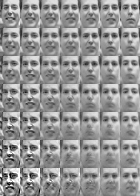
\includegraphics[width=.8\linewidth]{images/nf_frey_B400_E8000_N560_L2_H200_F2_C_manifold_8}
      \caption{Learned data manifold}
    \end{subfigure}
    \hspace{1em}
    \begin{subfigure}[b]{.4\linewidth}
      \centering
      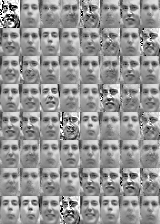
\includegraphics[width=.8\linewidth]{images/nf_frey_B400_E8000_N560_L2_H200_F2_C_sample_64}
      \caption{Random samples}
    \end{subfigure}
  \end{figure}
\end{frame}


\begin{frame}[fragile]{Experiments: Frey faces ($K = 8$)}
  \begin{figure}
    \centering
    \begin{subfigure}[b]{.4\linewidth}
      \centering
      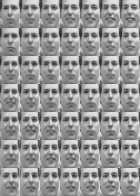
\includegraphics[width=.8\linewidth]{images/nf_frey_B400_E8000_N560_L2_H200_F8_C_manifold_8}
      \caption{Learned data manifold}
    \end{subfigure}
    \hspace{1em}
    \begin{subfigure}[b]{.4\linewidth}
      \centering
      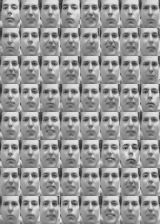
\includegraphics[width=.8\linewidth]{images/nf_frey_B400_E8000_N560_L2_H200_F8_C_sample_64}
      \caption{Random samples}
    \end{subfigure}
  \end{figure}
\end{frame}


\begin{frame}[fragile]{Experiments: Frey faces ($K = 16$)}
  \begin{figure}
    \centering
    \begin{subfigure}[b]{.4\linewidth}
      \centering
      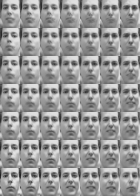
\includegraphics[width=.8\linewidth]{images/nf_frey_B400_E8000_N560_L2_H200_F16_C_manifold_8}
      \caption{Learned data manifold}
    \end{subfigure}
    \hspace{1em}
    \begin{subfigure}[b]{.4\linewidth}
      \centering
      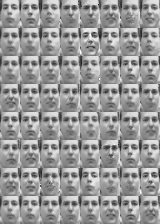
\includegraphics[width=.8\linewidth]{images/nf_frey_B400_E8000_N560_L2_H200_F16_C_sample_64}
      \caption{Random samples}
    \end{subfigure}
  \end{figure}
\end{frame}


\begin{frame}[fragile]{Experiments: Frey faces}
  \begin{center}
    \begin{tabular}{cc}
      \textbf{Model} & \textbf{ELBO} \\
      \hline
      VAE           & 519.72 \\
      NF ($K = 2$)  & 331.27 \\
      NF ($K = 8$)  & 410.03 \\
      NF ($K = 16$) & 415.49
    \end{tabular}
  \end{center}
\end{frame}


\begin{frame}[fragile]{Experiments: MNIST ($K = 2$)}
  \begin{figure}
    \centering
    \begin{subfigure}[b]{.4\linewidth}
      \centering
      %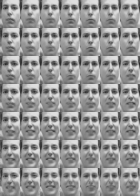
\includegraphics[width=\linewidth]{images/vae_frey_B100_E4000_N560_L2_H200_C_manifold_8}
      \caption{Learned data manifold}
    \end{subfigure}
    \hspace{1em}
    \begin{subfigure}[b]{.4\linewidth}
      \centering
      %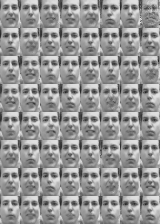
\includegraphics[width=\linewidth]{images/vae_frey_B100_E4000_N560_L2_H200_C_sample_64}
      \caption{Random samples}
    \end{subfigure}
  \end{figure}
\end{frame}


% 26
\begin{frame}[fragile]{Future directions}
  \begin{itemize}
  \item Investigate the effect of latent variable prior $p(z)$ and approximate
    posterior $q(z_K|x, \phi)$ on model performance.
  \item Try more complex prior distributions for the case when domain-specific
    knowledge is available, e.g. the data is multimodal.
  \item Apply normalizing flows to the problem of semi-supervised learning
    with generative models.
  \end{itemize}
\end{frame}


\begin{frame}[noframenumbering]{References}
  \bibliographystyle{apalike}
  \bibliography{references}
\end{frame}

\end{document}
